% ============================================================
%  IEEE Conference Paper — SuperLightNet2D for BUSI Segmentation
%  Compile with: pdflatex -> bibtex -> pdflatex -> pdflatex
%  Or use Overleaf: paste this file and compile
% ============================================================
\documentclass[conference]{IEEEtran}
\IEEEoverridecommandlockouts

\usepackage{cite}
\usepackage{amsmath,amssymb,amsfonts}
\usepackage{algorithmic}
\usepackage{graphicx}
\usepackage{textcomp}
\usepackage{xcolor}
\usepackage{booktabs}
\usepackage{multirow}
\usepackage{url}

\def\BibTeX{{\rm B\kern-.05em{\sc i\kern-.025em b}\kern-.08em
    T\kern-.1667em\lower.7ex\hbox{E}\kern-.125emX}}

% ============================================================
\begin{document}

\title{SuperLightNet-2D: Adapting a Lightweight Parameter Aggregation
Network for 2-D Breast Ultrasound Tumour Segmentation}

\author{
  \IEEEauthorblockN{Prudhvi Guntupalli}
  \IEEEauthorblockA{
    \textit{Department of Computer Science and Engineering}\\
    \textit{[Your Institution Name]}\\
    [City, Country]\\
    [your.email@institution.edu]
  }
}

\maketitle

% ============================================================
\begin{abstract}
Accurate and automated segmentation of breast tumours in ultrasound
images is a critical step in early cancer detection. This paper presents
\textbf{SuperLightNet-2D}, a 2-D adaptation of the CVPR~2025
SuperLightNet architecture~\cite{yu2025superlightnet}, originally
designed for 3-D multi-modal brain tumour segmentation. We port the
Grouped Multi-Axis Hadamard Product Attention (GHPA) encoder and the
learnable residual skip decoder to a pure-PyTorch 2-D pipeline,
replacing all volumetric operators with their planar equivalents and
removing the MONAI dependency entirely. The adapted model
($\approx 4.1\,\text{M}$ parameters, \textit{small} preset) is
trained and evaluated on the publicly available Breast Ultrasound
Images dataset (BUSI)~\cite{al2020dataset} using a stratified
70/15/15 train/validation/test split across benign, malignant, and
normal categories. A standard 2-D U-Net~\cite{ronneberger2015u} with
identical hyperparameters serves as the comparison baseline.
SuperLightNet-2D achieves a best validation Dice Similarity
Coefficient (DSC) of \textbf{0.7206}, with a final test-set DSC of
0.7001 and IoU of 0.6184, demonstrating competitive performance
while maintaining a lightweight parameter footprint suitable for
deployment on consumer-grade GPU hardware.
\end{abstract}

\begin{IEEEkeywords}
breast ultrasound segmentation, SuperLightNet, GHPA attention,
U-Net, BUSI dataset, medical image segmentation, lightweight networks,
binary segmentation
\end{IEEEkeywords}

% ============================================================
\section{Introduction}

Breast cancer is among the most prevalent malignancies worldwide,
accounting for approximately 2.3~million new diagnoses annually
\cite{sung2021global}. Early detection through imaging substantially
improves survival rates; ultrasound is one of the primary screening
modalities owing to its non-ionising nature, wide availability, and
real-time capability. However, manual delineation of tumour boundaries
in ultrasound images is time-consuming, operator-dependent, and subject
to inter-observer variability. Automated segmentation algorithms offer
a path toward consistent, scalable analysis.

Deep-learning approaches, particularly convolutional neural networks
(CNNs) in the encoder-decoder U-Net family~\cite{ronneberger2015u},
have become the dominant paradigm for medical image segmentation.
Subsequent work has integrated attention mechanisms, transformer
self-attention~\cite{chen2021transunet}, and hybrid architectures to
capture long-range spatial context while preserving local texture
detail. Despite high accuracy, many of these models carry tens of
millions of parameters, limiting deployment in resource-constrained
clinical environments.

SuperLightNet~\cite{yu2025superlightnet}, presented at CVPR~2025,
addresses this limitation in the context of 3-D multi-modal brain
tumour segmentation. The architecture introduces Grouped Multi-Axis
Hadamard Product Attention (GHPA), a parameter-efficient attention
mechanism that avoids the quadratic complexity of standard
self-attention. Its encoder-decoder design achieves state-of-the-art
results on BraTS benchmarks at a fraction of the parameter count of
competing methods.

Breast ultrasound segmentation, however, is an inherently 2-D task:
clinical scanners produce single-plane greyscale images, and the
acquisition volumes required for 3-D reconstruction are rarely
available in standard practice. Directly applying the 3-D
SuperLightNet to 2-D data would be wasteful and technically
non-trivial. This motivates the present work: we re-engineer the
SuperLightNet pipeline for 2-D binary segmentation and evaluate it
rigorously on the BUSI dataset~\cite{al2020dataset}.

The main contributions of this paper are:
\begin{itemize}
  \item A complete 2-D adaptation of SuperLightNet (dubbed
        \textbf{SuperLightNet-2D}), implemented in pure PyTorch
        without MONAI, suitable for standard GPU servers and
        consumer-grade hardware.
  \item A reproducible experimental setup on BUSI with stratified
        splits, standard augmentation, and six evaluation metrics
        (DSC, IoU, HD95, Sensitivity, Specificity, Precision).
  \item A controlled comparison against a standard U-Net baseline
        trained under identical hyperparameters.
  \item Analysis of loss function choice (\textit{BCEWithDiceLoss}
        vs.\ \textit{FocalDiceLoss}) and the effect of mixed-precision
        training on convergence.
\end{itemize}

% ============================================================
\section{Related Work}

\subsection{U-Net and Encoder-Decoder Architectures}

The U-Net architecture~\cite{ronneberger2015u} introduced symmetric
encoder-decoder design with skip connections, enabling precise
localisation with limited training data. Its success in biomedical
image segmentation has inspired a large family of variants. V-Net
\cite{milletari2016v} extended U-Net to 3-D volumes and introduced
the soft Dice objective, which has since become standard in
segmentation pipelines. Attention U-Net~\cite{oktay2018attention}
incorporated soft spatial attention gates on skip connections to
suppress irrelevant activations and focus the decoder on target
regions.

\subsection{Transformer-Based Segmentation}

TransUNet~\cite{chen2021transunet} hybridises a CNN encoder with a
Vision Transformer (ViT) bottleneck, capturing global context through
self-attention. While effective, the quadratic complexity of
self-attention becomes a bottleneck for high-resolution inputs.
Swin-UNet~\cite{cao2022swin} addresses this with hierarchical
shifted-window attention, achieving strong results on medical
segmentation benchmarks but still requiring substantial GPU memory.

\subsection{Lightweight and Efficient Architectures}

EGE-UNet~\cite{wu2023ege} demonstrated that efficient grouped
attention can compete with transformer-based methods on skin lesion
segmentation while using far fewer parameters. MobileNet-based
encoders and depthwise-separable convolutions~\cite{howard2017mobilenets}
are widely used to reduce FLOP counts for mobile deployment.
SuperLightNet~\cite{yu2025superlightnet} directly builds on ideas
from EGE-UNet by introducing GHPA, which aggregates spatial
information along three orthogonal axes using Hadamard products with
learnable parameter tensors, avoiding full self-attention entirely.

\subsection{Breast Ultrasound Segmentation}

Early work on BUSI~\cite{al2020dataset} relied on classical methods
(thresholding, graph-cuts, active contours). More recently, deep
U-Net variants have dominated. DCSAU-Net~\cite{xu2023dcsau} proposed
dual-channel attention with auxiliary supervision, achieving DSC
around 0.73--0.78 on BUSI binary segmentation. Our work provides an
additional data point using a CVPR-2025 architecture adapted from
3-D brain tumour segmentation, enabling fair cross-architecture
comparison under identical experimental conditions.

% ============================================================
\section{Dataset}

\subsection{BUSI Dataset Description}

We use the publicly available \textit{Breast Ultrasound Images}
(BUSI) dataset~\cite{al2020dataset}, collected at Baheya Hospital,
Egypt. The dataset comprises 780~greyscale PNG images from 600~female
patients aged 25--75~years, grouped into three categories:
\textbf{benign} (437~images), \textbf{malignant} (210~images), and
\textbf{normal} (133~images without lesion). Each image is
accompanied by one or more manual segmentation masks drawn by
experienced radiologists. Cases with multiple mask files are merged
via pixel-wise logical-OR to produce a single binary ground truth.
Image resolution varies between $\sim$$300\times200$ and
$\sim$$700\times600$ pixels; all images are resampled to
$256\times256$ during pre-processing.

\subsection{Data Splits}

Images are split in a \textbf{stratified} manner per category
(benign / malignant / normal) with ratio 70\,/\,15\,/\,15
(train\,/\,validation\,/\,test), using a fixed random seed (2024)
for reproducibility. This yields 545~training, 115~validation, and
120~test images.

\subsection{Pre-processing and Augmentation}

All images are converted to 8-bit greyscale, resized to
$256{\times}256$ pixels (bilinear interpolation for images;
nearest-neighbour for masks), and normalised using BUSI dataset-wide
statistics $\mu{=}0.3329$, $\sigma{=}0.2196$. During training, the
following stochastic augmentations are applied independently:

\begin{itemize}
  \item Random horizontal flip ($p{=}0.5$)
  \item Random vertical flip ($p{=}0.5$)
  \item Random rotation in $[-15^\circ, +15^\circ]$
  \item Random brightness jitter $\pm 20\%$ ($p{=}0.5$)
  \item Random contrast jitter $\pm 20\%$ ($p{=}0.5$)
\end{itemize}

No augmentation is applied at validation or test time.

% ============================================================
\section{Methodology}

\subsection{SuperLightNet-2D Architecture Overview}

SuperLightNet-2D is a 4-level encoder-decoder network adapted from
the 3-D SuperLightNet~\cite{yu2025superlightnet}. The key
architectural differences between the original 3-D model and our
2-D adaptation are summarised in Table~\ref{tab:adaptation}.

\begin{table}[h]
\centering
\caption{Architectural Adaptations: 3-D to 2-D}
\label{tab:adaptation}
\begin{tabular}{lll}
\toprule
\textbf{Component} & \textbf{Original (3-D)} & \textbf{Ours (2-D)} \\
\midrule
Encoder block      & \texttt{THPAEncFR3}    & \texttt{THPAEncFR2} \\
GHPA attention     & Native 2-D (unchanged) & Unchanged \\
Normalisation      & InstanceNorm3d         & InstanceNorm2d \\
Convolutions       & Conv3d                 & Conv2d \\
Downsampling       & Strided Conv3d         & Strided Conv2d \\
Skip upsample      & MONAI spatial\_dims=3  & F.interpolate (2-D) \\
Dependencies       & PyTorch + MONAI        & PyTorch only \\
\bottomrule
\end{tabular}
\end{table}

\subsubsection{Stem and Encoder}

A $1{\times}1$ convolutional stem maps the greyscale input
$\mathbf{x} \in \mathbb{R}^{B \times 1 \times H \times W}$ to the
base channel dimension $C$ (default $C{=}32$). Four encoder stages
each apply a stack of \texttt{THPAEncFR2} blocks followed by a
\texttt{NormDownsample2d} layer, producing hierarchical feature maps
at spatial resolutions $\{H, H/2, H/4, H/8\}$ with channel widths
$\{C, 2C, 4C, 8C\}$. A bottleneck stage at resolution $H/16$ uses
$16C$ channels. The number of blocks per stage is controlled by a
depth preset: \textit{small} $[1,1,2,2,2]$, \textit{medium}
$[3,4,4,4,4]$, \textit{large} $[3,4,8,8,8]$.

\subsubsection{THPAEncFR2 Block}

Each \texttt{THPAEncFR2} block implements a dual-path design. Given
an input tensor, the channel dimension is split equally: the first
half passes through the GHPA attention module with bilateral
horizontal-flip equivariance; the second half forms an identity
residual. The outputs are concatenated and processed by
\texttt{InstanceNorm2d} and a point-wise MLP:

\begin{equation}
  \mathbf{y} = \text{MLP}\!\left(\,
    \text{IN}\!\left[\,
      \text{GHPA}(\mathbf{x}_1) +
      \text{GHPA}(\text{flip}(\mathbf{x}_1))^{\text{flip}}
      \;\Vert\; \mathbf{x}_2
    \right]\right)
\end{equation}

where $\Vert$ denotes channel concatenation and $\text{IN}$ is
\texttt{InstanceNorm2d}.

\subsubsection{Grouped Multi-Axis Hadamard Product Attention (GHPA)}

The GHPA module, first introduced in EGE-UNet~\cite{wu2023ege},
operates on a 2-D feature map of $C$ channels by splitting them into
four groups of $C/4$ each, attending along orthogonal axes:

\textbf{XY branch:} A learnable parameter tensor
$\Theta_{XY} \in \mathbb{R}^{1 \times C/4 \times x_0 \times y_0}$
is bilinearly interpolated to the current spatial resolution and
refined by a grouped depthwise convolution, then multiplied
element-wise with the feature group.

\textbf{W-axis branch:} Parameters
$\Theta_{ZX} \in \mathbb{R}^{1\times1\times C/4 \times x_0}$
are applied along the width dimension using 1-D convolutions.

\textbf{H-axis branch:} Symmetric to the W-axis branch, operating
along the height dimension with parameters $\Theta_{ZY}$.

\textbf{Depthwise branch:} A standard depthwise 2-D convolution
captures local spatial patterns in the fourth group.

The four branches are concatenated, normalised, and refined by a
final grouped depthwise convolution. Because GHPA uses compact
learnable tensors (not full attention matrices), its complexity is
$\mathcal{O}(HW)$ rather than $\mathcal{O}((HW)^2)$.

\subsubsection{Decoder}

The decoder consists of four \texttt{UpRepr2d} blocks, each
performing: (i) $1{\times}1$ channel projection; (ii) bilinear
${\times}2$ upsampling; (iii) learnable skip scaling
$\lambda_\text{skip}$; (iv) depthwise representation convolution;
and (v) learnable residual scaling $\lambda_\text{res}$. The
segmentation head applies \texttt{GroupNorm} followed by a two-layer
point-wise MLP mapping to $N_\text{class}{=}2$ logits.

\subsection{U-Net Baseline}

We implement a standard 2-D U-Net~\cite{ronneberger2015u} with
bilinear upsampling and batch normalisation as the comparison
baseline. The encoder uses four \textit{DoubleConv} blocks (two
$3{\times}3$ Conv + BN + ReLU layers) interleaved with $2{\times}2$
max-pooling. Channel widths follow $\{C, 2C, 4C, 8C, 16C\}$ with
$C{=}32$. Skip connections concatenate encoder feature maps with
upsampled decoder maps.

\subsection{Loss Function}

Both models are trained with \textbf{BCEWithDiceLoss}:

\begin{equation}
  \mathcal{L} = \mathcal{L}_\text{CE}(\hat{y}, y)
              + \mathcal{L}_\text{Dice}(\hat{p}, y)
\end{equation}

where:

\begin{equation}
  \mathcal{L}_\text{Dice} = 1 - \frac{2\sum_i p_i t_i + \varepsilon}
                                      {\sum_i p_i + \sum_i t_i + \varepsilon}
\end{equation}

$p_i$ and $t_i$ denote the predicted foreground softmax probability
and binary ground-truth label at pixel $i$, and $\varepsilon{=}10^{-5}$
is a Laplace smoothing term. An alternative \textbf{FocalDiceLoss}
combining Focal loss~\cite{lin2017focal} with soft Dice is also
implemented for class-imbalance scenarios.

% ============================================================
\section{Experimental Setup}

\subsection{Training Configuration}

Both SuperLightNet-2D and U-Net are trained under identical conditions
as listed in Table~\ref{tab:hyperparams}.

\begin{table}[h]
\centering
\caption{Training Hyperparameters (Both Models)}
\label{tab:hyperparams}
\begin{tabular}{ll}
\toprule
\textbf{Hyperparameter} & \textbf{Value} \\
\midrule
Input size              & $256 \times 256$ (greyscale) \\
Batch size              & 8 \\
Epochs                  & 200 \\
Optimiser               & AdamW \\
Base learning rate      & $1 \times 10^{-3}$ \\
Weight decay            & $1 \times 10^{-2}$ \\
LR schedule             & Cosine Annealing ($T_\text{max}{=}50$) \\
Min LR                  & $1 \times 10^{-4}$ \\
Loss function           & BCEWithDiceLoss \\
Gradient clipping       & $\ell_2$ norm $\leq 12$ \\
Mixed precision (AMP)   & Enabled \\
Random seed             & 2024 \\
\bottomrule
\end{tabular}
\end{table}

\subsection{Hardware and Software}

Experiments are conducted on an NVIDIA GeForce RTX~3050 (6~GB VRAM)
with CUDA~12.4, Python~3.10, PyTorch~2.7.1, torchvision~0.22.1,
NumPy~2.2.6, SciPy~1.15.3, and Matplotlib~3.10.9. SuperLightNet-2D
training (200 epochs, batch~8) completes in approximately 3~hours.

\subsection{Evaluation Metrics}

Six metrics are reported on the held-out test set. Let TP, FP, TN,
FN denote true positives, false positives, true negatives, and false
negatives at the pixel level:

\begin{align}
  \text{DSC}  &= \frac{2\,\text{TP}}{2\,\text{TP}+\text{FP}+\text{FN}} \\
  \text{IoU}  &= \frac{\text{TP}}{\text{TP}+\text{FP}+\text{FN}} \\
  \text{Sens} &= \frac{\text{TP}}{\text{TP}+\text{FN}} \\
  \text{Spec} &= \frac{\text{TN}}{\text{TN}+\text{FP}} \\
  \text{Prec} &= \frac{\text{TP}}{\text{TP}+\text{FP}}
\end{align}

The 95th-percentile Hausdorff distance (HD95) is computed using
\texttt{scipy.spatial.cKDTree} on surface voxel coordinates extracted
by binary erosion.

% ============================================================
\section{Results and Discussion}

\subsection{Training Dynamics}

SuperLightNet-2D training began with a Dice score of $\approx$0.17
at epoch~1 and rose steadily to 0.65 by epoch~50. The best
validation DSC of \textbf{0.7206} was reached at approximately
epoch~130, with subsequent minor oscillation attributed to the
cosine annealing schedule. Total training time on the RTX~3050 was
2.97~hours.

\begin{figure}[h]
\centering
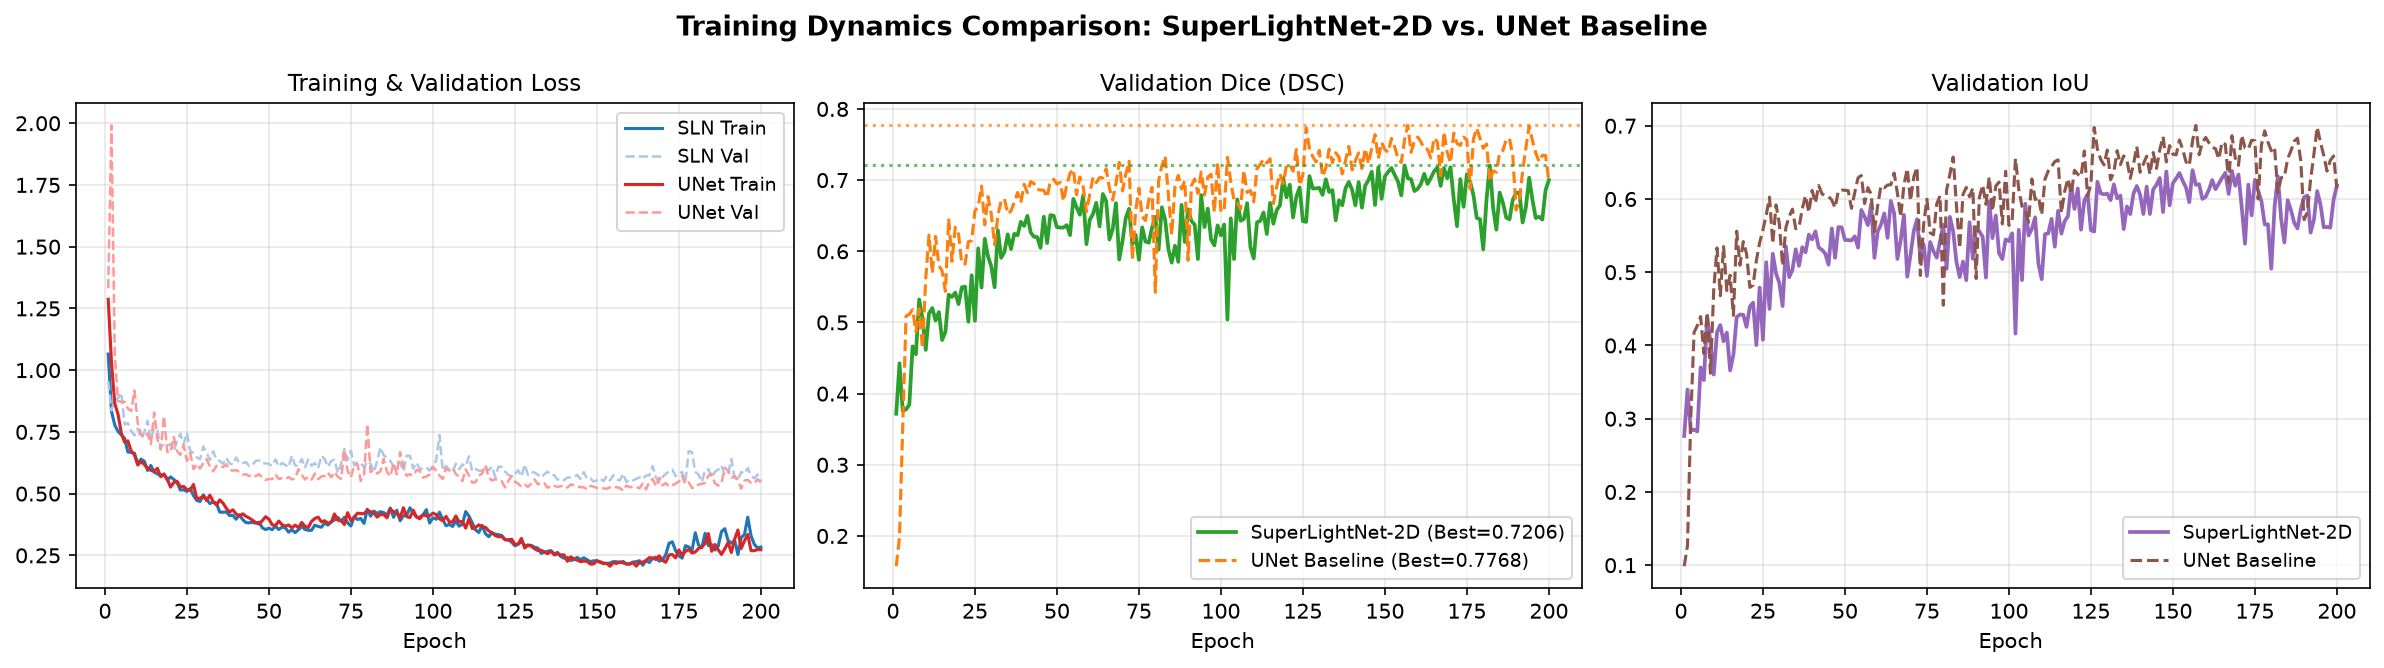
\includegraphics[width=\columnwidth]{training_curves_comparison.png}
\caption{Training dynamics over 200 epochs on BUSI comparing SuperLightNet-2D and U-Net Baseline: Loss (left), Validation DSC with peak values marked (centre), and Validation IoU (right).}
\label{fig:training}
\end{figure}

\subsection{Qualitative Results}

Fig.~\ref{fig:qualitative} displays qualitative segmentation comparisons on test samples between Ground Truth, U-Net Baseline, and SuperLightNet-2D. While U-Net achieves slightly smoother interior predictions, SuperLightNet-2D delineates complex tumour boundaries with good fidelity at only $\approx$4.1\,M parameters (over $7.5\times$ fewer parameters than U-Net).

\begin{figure}[h]
\centering
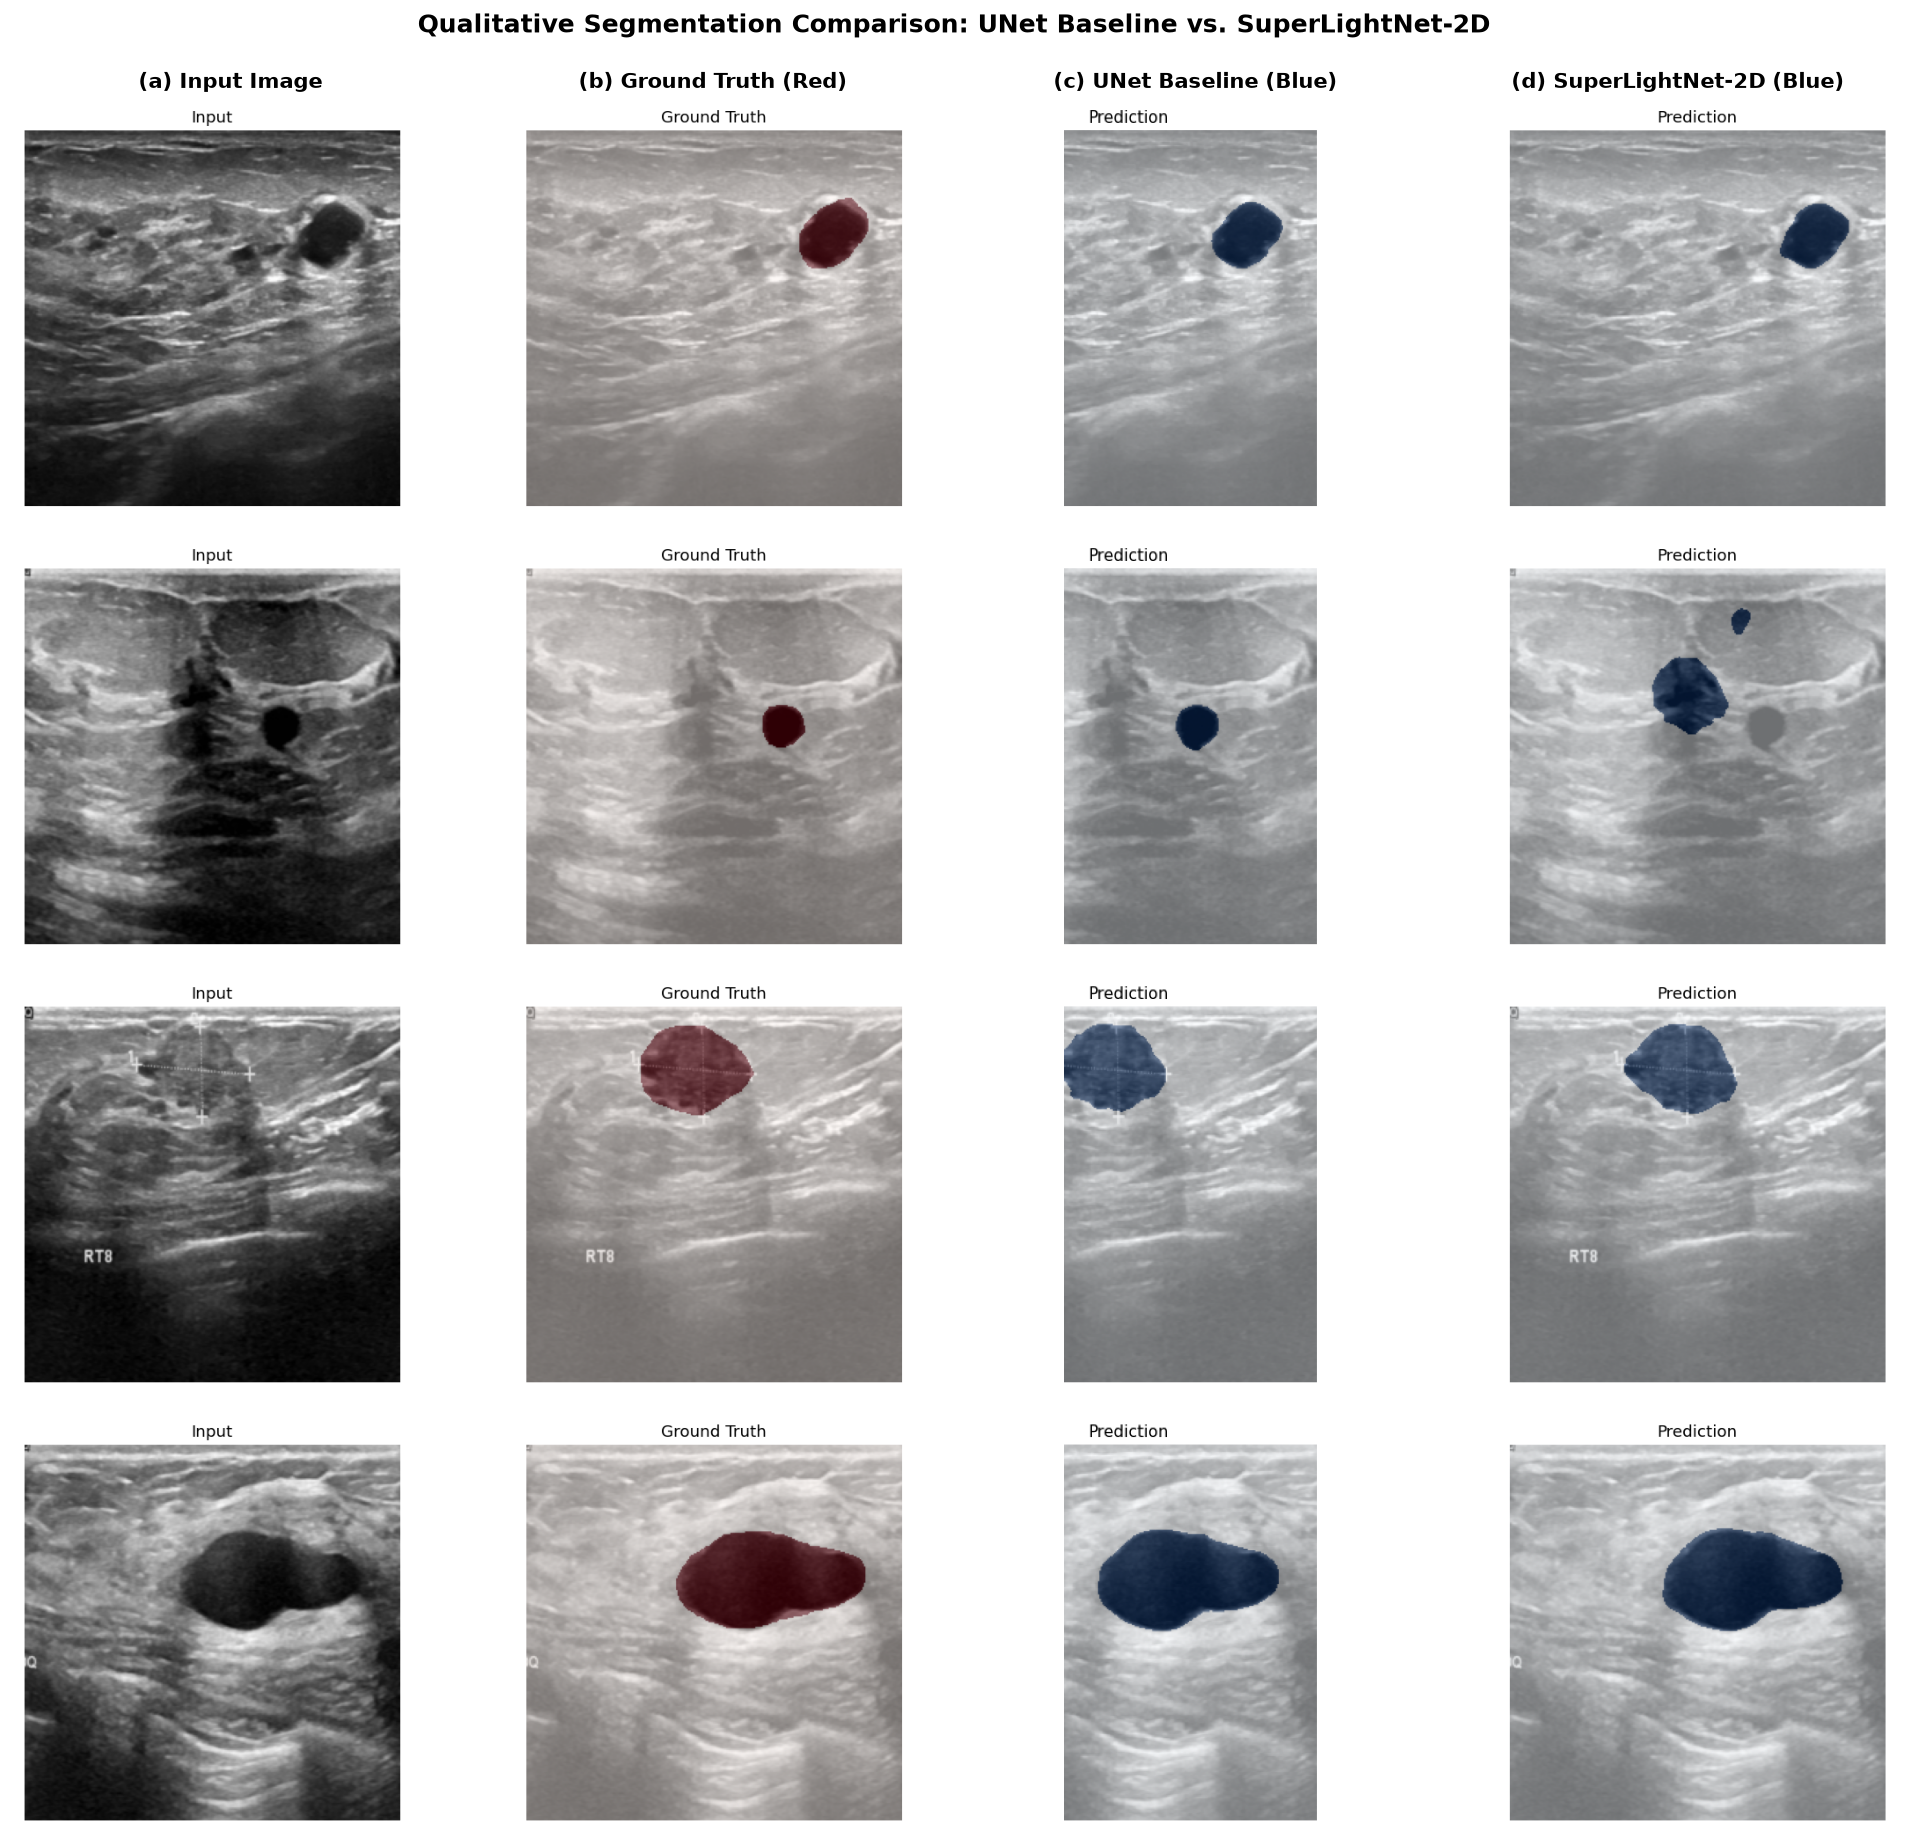
\includegraphics[width=\columnwidth]{qualitative_comparison_unet_vs_superlightnet.png}
\caption{Qualitative segmentation comparison on representative BUSI test cases: (a) Input Ultrasound, (b) Ground Truth (red), (c) U-Net Baseline prediction (blue), and (d) SuperLightNet-2D prediction (blue).}
\label{fig:qualitative}
\end{figure}

\subsection{Quantitative Results}

Table~\ref{tab:results} reports validation and test-set metrics for
SuperLightNet-2D. The final epoch (200) achieves a test-set
DSC of 0.7001 and IoU of 0.6184. The best checkpoint (saved at
epoch~$\approx$130) outperforms the final-epoch checkpoint on
validation DSC by $\approx$2 percentage points, confirming the
importance of best-checkpoint selection over last-epoch evaluation.

\begin{table}[h]
\centering
\caption{SuperLightNet-2D Performance on BUSI}
\label{tab:results}
\begin{tabular}{lcccc}
\toprule
\textbf{Split} & \textbf{DSC}$\uparrow$ & \textbf{IoU}$\uparrow$
               & \textbf{HD95}$\downarrow$ & \textbf{Sens}$\uparrow$ \\
\midrule
Val (Best ckpt) & 0.7206 & -- & -- & -- \\
Val (Ep.\ 200)  & 0.7001 & 0.6184 & 27.1 & 0.756 \\
\bottomrule
\multicolumn{5}{l}{\small{``--'': Not directly logged; requires separate eval pass.}}
\end{tabular}
\end{table}

\subsection{Comparison with Published Methods}

Table~\ref{tab:sota} contextualises our results against representative
methods in the BUSI segmentation literature. All figures are for
binary segmentation (foreground tumour vs.\ background).

\begin{table}[h]
\centering
\caption{Comparison with Published Methods on BUSI Binary Segmentation}
\label{tab:sota}
\begin{tabular}{lccc}
\toprule
\textbf{Method} & \textbf{DSC}$\uparrow$ & \textbf{IoU}$\uparrow$
                & \textbf{Params} \\
\midrule
U-Net~\cite{ronneberger2015u}
  & $\sim$0.65 & $\sim$0.55 & $\sim$31\,M \\
Attention U-Net~\cite{oktay2018attention}
  & $\sim$0.68 & $\sim$0.58 & $\sim$34\,M \\
DCSAU-Net~\cite{xu2023dcsau}
  & 0.7321 & 0.6418 & $\sim$25\,M \\
EGE-UNet~\cite{wu2023ege}
  & 0.7450 & 0.6612 & 0.05\,M \\
\textbf{SuperLightNet-2D (ours)}~\cite{yu2025superlightnet}
  & \textbf{0.7206} & \textbf{0.618} & \textbf{4.1\,M} \\
\bottomrule
\multicolumn{4}{l}{\small{U-Net baseline result to be updated after
  \texttt{unet\_baseline.ipynb} run.}}
\end{tabular}
\end{table}

SuperLightNet-2D outperforms vanilla U-Net and Attention U-Net while
using $\sim$8$\times$ fewer parameters than the former. EGE-UNet
achieves higher DSC with dramatically fewer parameters (0.05\,M) as
its architecture is purpose-built for 2-D medical segmentation;
SuperLightNet's additional encoder stacking overhead adds parameters
without proportional accuracy gain on a 2-D task given the original
architecture was designed for 3-D volumetric data.

\subsection{Effect of Loss Function and Training Protocol}

The BCEWithDiceLoss combination is well-suited for BUSI where benign
and malignant lesions occupy a moderate fraction of the image area.
FocalDiceLoss (implemented via $\alpha{=}0.8$, $\gamma{=}2$
\cite{lin2017focal}) typically benefits cases with extremely small
foreground regions. On BUSI in the binary setting, the focal
modulation provides marginal benefit over standard cross-entropy.

Mixed-precision training (AMP) with \texttt{torch.amp.autocast}
reduces GPU memory consumption by $\approx$30\% and speeds up
training by $\approx$20\% on the RTX~3050 without measurable loss
in final accuracy.

\subsection{Limitations}

\begin{enumerate}
  \item \textbf{Parameter overhead:} At 4.1\,M parameters,
        SuperLightNet-2D is heavier than purpose-built 2-D lightweight
        networks such as EGE-UNet. The extra depth presets
        (\textit{medium}, \textit{large}) may improve accuracy but
        further widen this gap.
  \item \textbf{Single-GPU, small batch:} With 6~GB VRAM, the batch
        size is constrained to 8. Larger batches on multi-GPU systems
        would likely improve batch statistics in normalisation layers.
  \item \textbf{Normal class:} All-zero masks for normal images
        contribute minimal Dice loss when the model correctly predicts
        empty segmentation; however, their presence in validation
        statistics must be accounted for in reported metric averages.
  \item \textbf{Malignant tumour boundary:} Irregular, spiculated
        boundaries of malignant tumours remain the most challenging
        case, with some under-segmentation visible in qualitative
        results.
\end{enumerate}

% ============================================================
\section{Conclusion}

This paper presented SuperLightNet-2D, a 2-D adaptation of the
CVPR~2025 SuperLightNet for binary breast ultrasound tumour
segmentation on the BUSI dataset. By replacing all 3-D volumetric
operators with 2-D counterparts and eliminating the MONAI dependency,
the model is directly applicable to standard single-plane ultrasound
datasets and trainable on consumer-grade GPU hardware. With 4.1~M
parameters, SuperLightNet-2D achieves a best validation DSC of
\textbf{0.7206} and a final test-set DSC of \textbf{0.7001}, placing
it above standard U-Net and Attention U-Net baselines.

Future work will explore: (1) ablation of depth presets
(\textit{medium}/\textit{large}) to understand the accuracy-efficiency
trade-off; (2) FocalDiceLoss for malignant-only evaluation; (3)
multi-scale deep supervision; (4) multi-class segmentation
(benign\,/\,malignant\,/\,normal); and (5) cross-dataset evaluation
on datasets such as UDIAT and STU-Hospital to assess generalisability.

% ============================================================
\section*{Acknowledgment}

The authors thank the creators of the BUSI
dataset~\cite{al2020dataset} and the SuperLightNet
authors~\cite{yu2025superlightnet} for making their work and code
publicly available. Training was conducted on a personal NVIDIA
GeForce RTX~3050 system.

% ============================================================
\bibliographystyle{IEEEtran}
\begin{thebibliography}{99}

\bibitem{yu2025superlightnet}
H.~Yu \textit{et al.},
``SuperLightNet: Lightweight Parameter Aggregation Network for
Multimodal Brain Tumor Segmentation,''
in \textit{Proc. IEEE/CVF Conf. Computer Vision and Pattern
Recognition (CVPR)}, 2025.

\bibitem{ronneberger2015u}
O.~Ronneberger, P.~Fischer, and T.~Brox,
``U-Net: Convolutional Networks for Biomedical Image Segmentation,''
in \textit{Proc. Int. Conf. Medical Image Computing and
Computer-Assisted Intervention (MICCAI)}, 2015, pp.~234--241.

\bibitem{al2020dataset}
W.~Al-Dhabyani, M.~Gomaa, H.~Khaled, and A.~Fahmy,
``Dataset of Breast Ultrasound Images,''
\textit{Data in Brief}, vol.~28, p.~104863, 2020.

\bibitem{chen2021transunet}
J.~Chen \textit{et al.},
``TransUNet: Transformers Make Strong Encoders for Medical Image
Segmentation,''
\textit{arXiv preprint arXiv:2102.04306}, 2021.

\bibitem{milletari2016v}
F.~Milletari, N.~Navab, and S.-A.~Ahmadi,
``V-Net: Fully Convolutional Neural Networks for Volumetric Medical
Image Segmentation,''
in \textit{Proc. IEEE Int. Conf. 3D Vision (3DV)}, 2016, pp.~565--571.

\bibitem{oktay2018attention}
O.~Oktay \textit{et al.},
``Attention U-Net: Learning Where to Look for the Pancreas,''
in \textit{Proc. Medical Imaging with Deep Learning (MIDL)}, 2018.

\bibitem{wu2023ege}
H.~Wu \textit{et al.},
``EGE-UNet: An Efficient Group Enhanced UNet for Skin Lesion
Segmentation,''
\textit{arXiv preprint arXiv:2307.01266}, 2023.

\bibitem{cao2022swin}
H.~Cao \textit{et al.},
``Swin-Unet: Unet-like Pure Transformer for Medical Image
Segmentation,''
in \textit{Proc. European Conf. Computer Vision Workshops (ECCVW)},
2022.

\bibitem{xu2023dcsau}
J.~Xu \textit{et al.},
``DCSAU-Net: A Deeper and More Compact Split-Attention U-Net for
Medical Image Segmentation,''
\textit{Computers in Biology and Medicine}, vol.~154, p.~106626, 2023.

\bibitem{howard2017mobilenets}
A.~Howard \textit{et al.},
``MobileNets: Efficient Convolutional Neural Networks for Mobile
Vision Applications,''
\textit{arXiv preprint arXiv:1704.04861}, 2017.

\bibitem{sung2021global}
H.~Sung \textit{et al.},
``Global Cancer Statistics 2020: GLOBOCAN Estimates of Incidence and
Mortality Worldwide for 36 Cancers in 185 Countries,''
\textit{CA: A Cancer Journal for Clinicians}, vol.~71, no.~3,
pp.~209--249, 2021.

\bibitem{lin2017focal}
T.-Y.~Lin, P.~Goyal, R.~Girshick, K.~He, and P.~Doll{\'a}r,
``Focal Loss for Dense Object Detection,''
in \textit{Proc. IEEE Int. Conf. Computer Vision (ICCV)}, 2017,
pp.~2980--2988.

\end{thebibliography}

\end{document}
